%\chapter{Acceptance testing with FitNesse}

% Hickl

\chapter{Systematic Generation of acceptance tests that are executable with FitNesse}
\label{sec:topic_2}

\section{Introduction}\label{sec:topic_2_intro}

This chapter focusses on the creation of acceptance tests that are automatically executable using the tool \textit{FitNesse}.
In this first section of the chapter the reason for using this approach is discussed.
Furthermore, the general features of \textit{FitNesse} as well as the needed artefacts like Fit-tables are explained.
An article that focuses on the topic of creating acceptance tests that are executable with \textit{FitNesse} was provided by the supervisors of the seminar.
Section \ref{sec:literature-search} documents the literature search used to find a different approach.
The two articles are then described in the sections \ref{sec:el-attar} and \ref{sec:longo}.
Moreover, for a better understanding of the presented approaches these chapters include the execution of them on the \textit{MovieManager}.
The following section \ref{sec:comparison} includes the comparison of the two approaches using a synthesis matrix.
Section \ref{sec:topic_2_conclusion} provides a Conclusion including the most important insights of the process and an assessment in which situations the approaches might be suitable.

During the software engineering process communication between the developers and the customers is a crucial factor for the success of the product.
A problem for the communication is the different use of documents by the two main stakeholders:
Customers describe their requirements in natural language whereas the developers create code.
Natural language can often be interpreted in different ways, which can lead to unwanted results.
And whereas code is more precise, it is often too technical for the customer.
Therefore, artefacts are needed that are more precise than natural language and can easily be transformed into code.

One such artefact is a \textit{Fit-table}. 
These tables store easily readable information about acceptance test cases and can be fully automatically executed using the testing tool \textit{FitNesse} \cite{fitnesse}.
Creating \textit{Fit-tables} before the development of the software can help the developers to understand the requirements of the customer by implementing the necessary functionality to pass the acceptance tests.
Thus the customers receive a software that satisfies all their mentioned requirements.
\textit{FitNesse} supports the creation and maintenance of \textit{Fit-tables} as well as the automated execution of the tests represented by the tables.
To make this possible \textit{Fixture-Classes} are needed.
These classes connect the input values from the \textit{Fit-tables} to the \textit{System-under-test} and are executed by \textit{FitNesse}.
An overview of the data exchange during the process is shown in figure \ref{fig:overview-fitnesse} on the next page.
The specific steps are explained in the following:

After the user chooses to execute a set of Fit-tables in \textit{FitNesse}, \textit{FitNesse} executes the Fixture-Classes that belong to the selected tables.
These tables can contain two types of values: Input values and expected output values.
The \textit{Fixture-Class} creates an instance of the \textit{System-under-test} and then transfers the input values into it.
Then it extracts the resulting output values from the \textit{System-under-test} and returns them to \textit{FitNesse}.
These extracted output values are then automatically compared by \textit{FitNesse} to the expected output values from the Fit-tables.
If they are the same, the test was successful and the entry of the table receives the colour \textit{Green}.
Otherwise, the affected part of the test failed and the entry receives the colour \textit{Red}.

\begin{figure}[H]
	\centering
	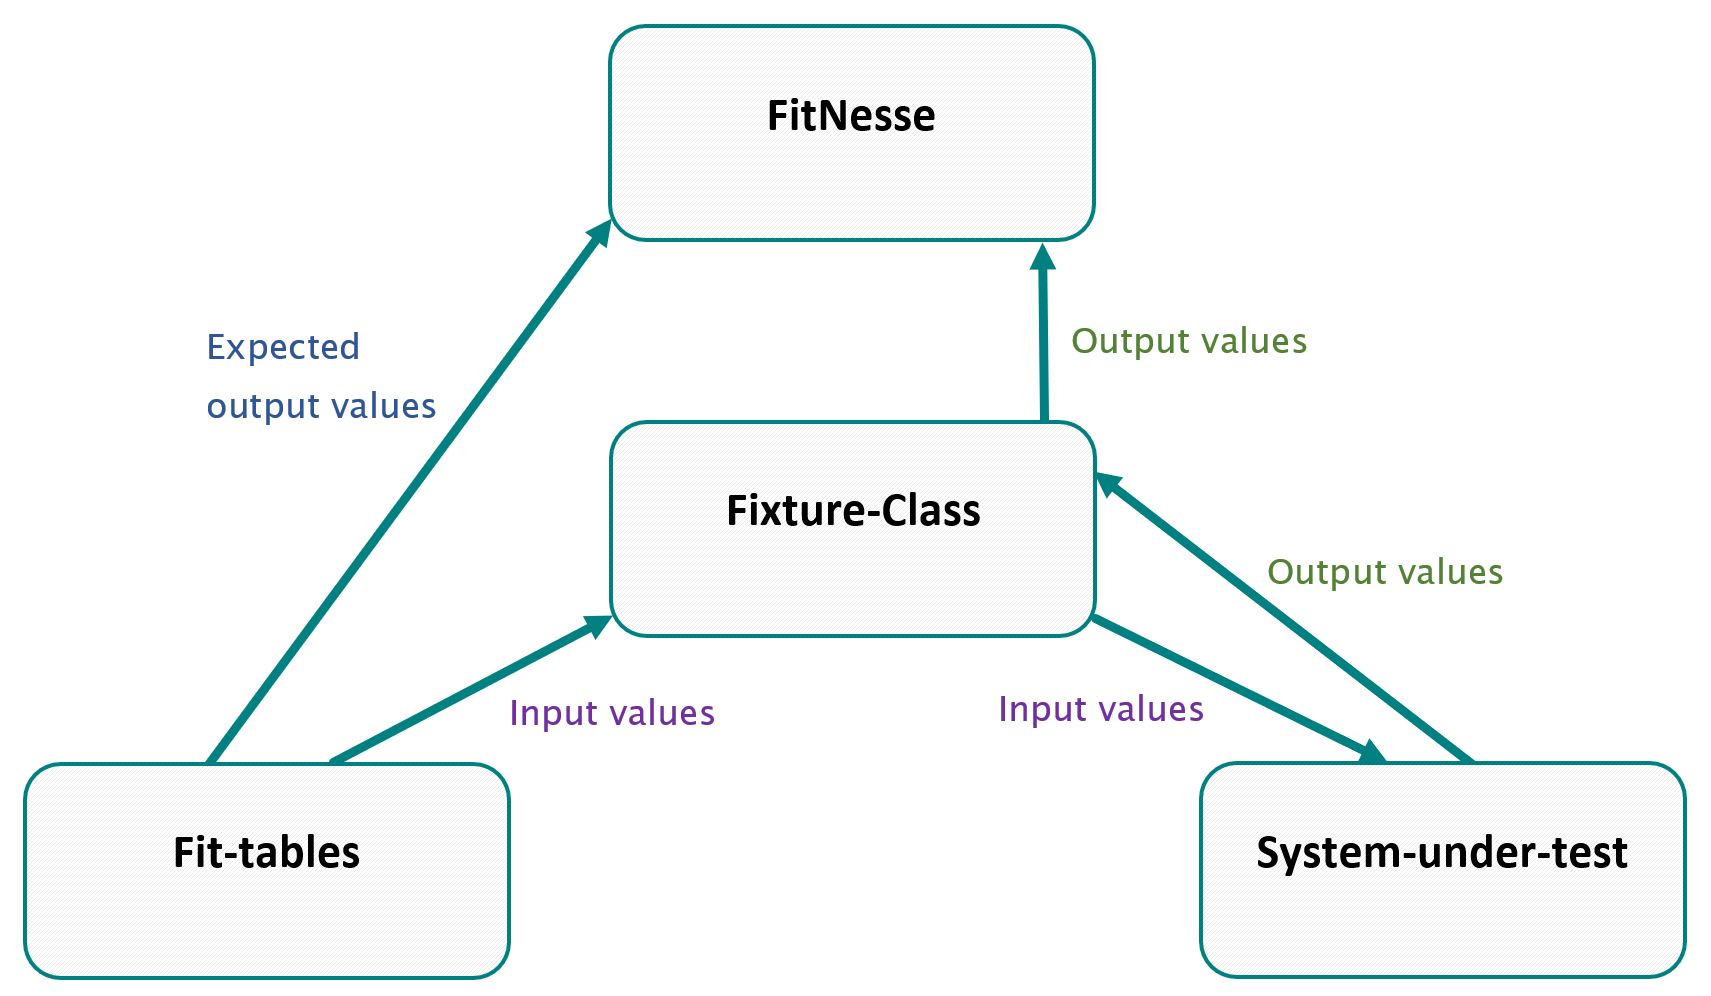
\includegraphics[width=.75\textwidth]{../images/fitnesse-overview.png}
	\caption{Overview of the data exchange in the execution of \textit{Fit-tables} with \textit{FitNesse}. The Fit-tables can be created and maintained in FitNesse.}
	\label{fig:overview-fitnesse}
\end{figure}


\section{Literature search}
\label{sec:literature-search}

The literature search consisted of a search-term-based search as well as forward- and backward-snowballing.
As start article the work of El-Attar and Smith \cite{el-attar} was given by the supervisor of this seminar.
This article presents an approach to create acceptance tests that can be automatically executed using \textit{FitNesse}.
To find more and possibly different approaches the search question was chosen to be:

\begin{center}
\textit{
 Which approaches to systematically generate acceptance tests that are executable with \textit{FitNesse} exist in the literature?
}
\end{center}

\textit{ACM Digital Library} \cite{acm}, \textit{IEEE Xplore} \cite{ieee}, \textit{Springer Link} \cite{springer} and \textit{Science Direct} \cite{elsevier} were used as search platforms as they are the most common platforms in the field of computer science.
The relevance criteria were chosen as follows:
\begin{itemize}
	\item \textit{Criterion 1:} The article describes an approach to systematically generate acceptance tests that are executable with \textit{FitNesse} \textit{or} gives an overview on the use of \textit{FitNesse} in software engineering.
	
	This criterion was chosen to find approaches that are specific to the subject of this chapter.
	Articles that give an overview over the use of \textit{FitNesse} were also accepted because of their potential to classify the found approaches.
	
	\item \textit{Criterion 2:} The article was not published before the year 2009 which is the year that the article by El-Attar and Smith was published.
	
	This criterion was chosen to get a more recent approach than the start article which was by the creation of this chapter already more than 10 years old.
\end{itemize}

Table \ref{fig:lit-search-fitnesse} on the next page provides an overview for the search-term-based literature search.
As search terms the terms \enquote{acceptance test} and \enquote{FitNesse} were chosen.
These search terms turned out to be specific enough to fit only a manageable amount of articles.
The search resulted in eight relevant articles of which six presented an approach and two gave an overview over the use of \textit{FitNesse}.
Both snowballing searches from the start articles did not result in any more relevant articles that were not already found by the search-term-based search.
The backward-snowballing did not result in any relevant articles due to their publishing date and hence not passing Criterion 2.
One relevant article was found during the forward-snowballing that was already found by the search-term-based search on the platform Springer Link.

\begin{table}[H]
	\caption{Overview of the search-term-based literature search.}
	
	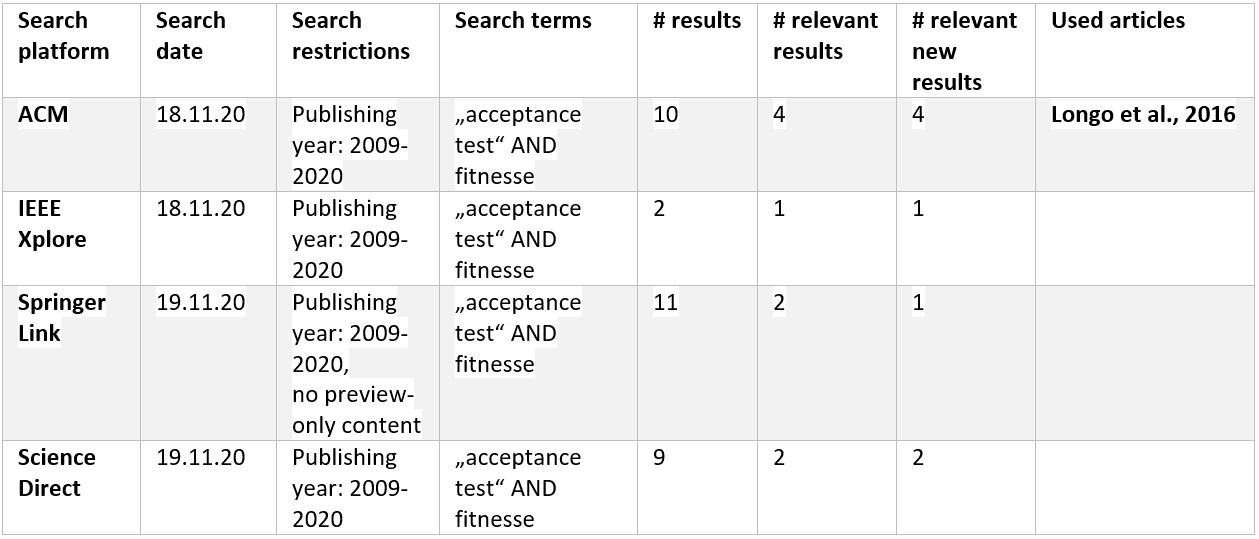
\includegraphics[width=\textwidth]{../images/LitSearchFitnesse.png} 
	
	\label{fig:lit-search-fitnesse}
\end{table}


The articles that gave an overview over the use of FitNesse were not specific about any approaches and only provided general information.
Therefore, none of these articles was used.
As a second approach to compare to the start article, the work by Longo et al. \cite{longo} was chosen.
This article also describes an approach to create acceptance tests that can be automatically executed by \textit{FitNesse}.
The presented approach differs from the approach of the article by El-Attar and Smith in its use of artefacts.
Also it was created by different authors and was published in 2016, so it is a much more recent approach.


\section{Approach 1: Developing comprehensive acceptance tests from Use Cases and robustness diagrams}
\label{sec:el-attar}

\subsection{Description}

El-Attar and Smith \cite{el-attar} introduce an approach to create acceptance tests that can be automatically executed using \textit{FitNesse.}
Their approach is targeted at larger software projects that use a model-based approach such as the use of UML models. 
It was created such that a non-technical person (e.g. a Business Analyst) can execute it during the early phases of the development of the software.
This makes it possible for the developers to follow the approach of Acceptance-Test-Driven-Development (ATDD) because of the possibility of executing the acceptance tests at any time during the development process.
ATDD helps the developers during the development process to evaluate which requirements are already implemented and  which are yet to be implemented.

The approach starts with use case models and domain models as initial artefacts.
During the whole process of creating the acceptance tests every step is performed completely manually.
The execution of the final acceptance tests is done fully automatically by the tool \textit{FitNesse}.
To help with traceability during the approach the authors created a tool called UCAT.
This tool does not provide any automation support but allows the user to create use case models and \textit{Fit-tables}.
These artefacts can be linked within UCAT which helps to determine which use cases resulted in which acceptance tests.
Figure \ref{fig:overview-el-attar} shows the rough structure of the approach.
The exact steps of the approach are described in the following:

\begin{figure}
	\centering
	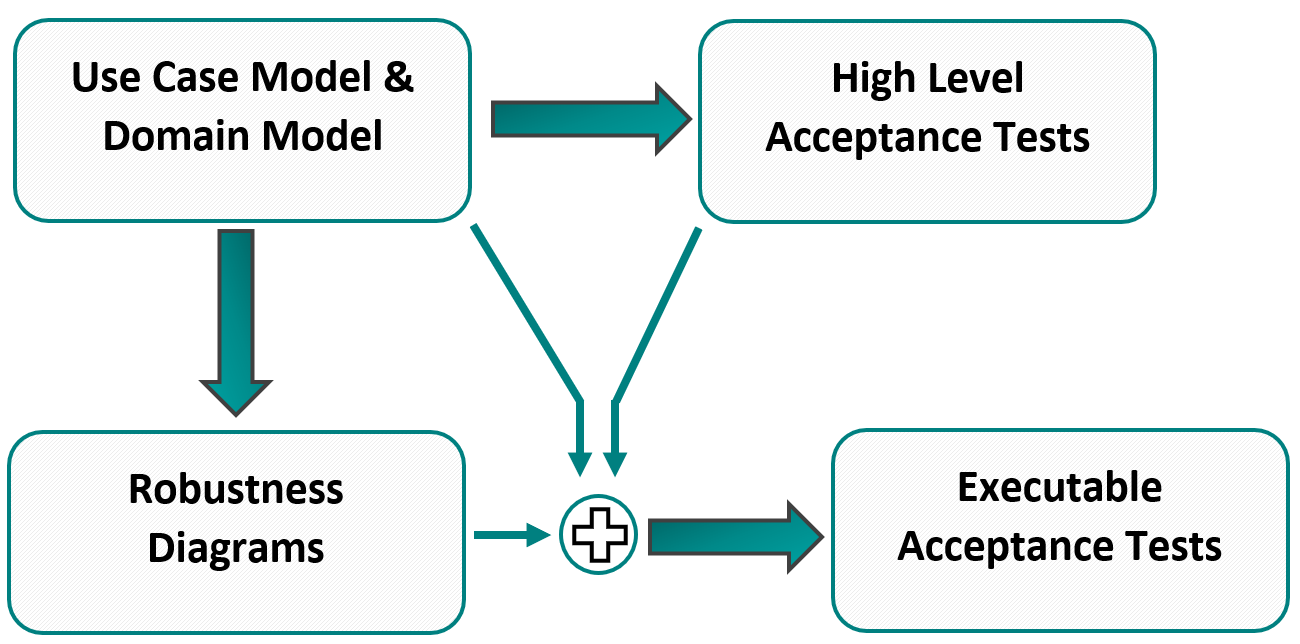
\includegraphics[width=.8\textwidth]{../images/ElAttarProcess.png}
	\caption{Overview of the steps in the approach of El-Attar and Smith.}
	\label{fig:overview-el-attar}
\end{figure}

In the first step of the approach \textbf{High-Level-Acceptance-Tests (HLATs)} are created.
For this a domain model and a Use Case model with Use case descriptions is required in the approach.
HLATs are more informal than an executable acceptance test which helps the analyst to be as flexible as possible in describing the acceptance tests at this early stage.
Commonly Use Cases contain Use Case descriptions from which the flows of the Use Case can be extracted.
HLATs describe the system's expected behaviour during all of the flows of the use cases from the Use Case model.
Necessary Pre-Conditions and triggers for the flows are also extracted from the Use Case description while the inputs for the flows can be extracted from the domain model.
Expected test results are also denoted in the HLATs.
At this point they do not need to contain specific values and can be written in natural language.
The general structure of a HLAT is shown in Table 1.2.


\begin{table}[H]
	\begin{small}
	\caption{General structure of a HLAT.}
	\renewcommand{\arraystretch}{1.5}
	\begin{tabularx}{\textwidth}{X|X|X}
		\hline
  		\textbf{Test ID} & \textbf{Description} & \textbf{Expected \newline Result} \\
  		\hline
  		Name of the Use Case \& the flow & Preconditions: \newline Inputs: & Expected result in natural language \\
  		\hline
 	\end{tabularx}
 	\renewcommand{\arraystretch}{1}
 	\label{fig:1}
 	\end{small}	
\end{table}


After the creation of the HLATs a robustness analysis is performed.
To achieve this, for every use case a \textbf{robustness diagram} is created.
These diagrams combine the use cases from the use case model with the objects from the domain model.
They contain actors and entities as well as boundary- and control-objects.
For each use case all involved objects and the connections between the objects are displayed.
The involved objects and the communication between them is extracted from the Use Case description.
During the creation of the robustness diagrams necessary \textit{objects} or \textit{attributes of objects} may be identified that are not already part of the domain model.
These should be added to the domain model.
Also missing steps or preconditions in the Use Case description might be found.
If this is the case, the Use Case descriptions should also be updated.
After this step the HLATs should be adapted to fit the updated domain model and Use Case descriptions.

In the last step all the existing artefacts (possibly except the domain models) are used to create the final product of the approach: \textbf{Executable Acceptance Tests (EATs)}.
These acceptance tests are in the form of specific \textit{Fit-tables}.
To achieve this, the HLATs have to be divided into smaller steps using the information about the Usage Scenario from the related use case description.
This step requires human judgment and is not further described.
For each of these steps the control flow in the robustness diagram gets traced.
In this process the objects and attributes of each step's input, preconditions, outputs and postconditions are determined.
These where before stated in natural language in the HLAT and are exchanged in the EAT with more concrete objects and attributes.
The steps combined with the corresponding control flow are manually converted into \textit{Fit-tables}.
\textit{Fit-tables} used in this approach are either \textit{ActionFixtures}, \textit{RowFixtures} or \textit{ColumnFixtures} \cite{Fit-tables}.
These types of \textit{Fit-tables} can be fully automatically executed using the tool \textit{FitNesse}.
The domain models are ideally not required if the steps before where executed properly because the information from the domain models should already be part of the use case descriptions.

Due to the fact that the approach of creating the acceptance tests is done completely manually, the quality of the resulting acceptance tests depends highly on the experience and skills of the person executing the approach.
Therefore, the authors state that an evaluation would be beyond the limitations of their work.
However, they provide a case example by applying the approach to the software \textit{RestoMapper}.
This example is not part of this work because in the following section the execution of the approach is presented with the application \textit{Movie Manager} that is used throughout this whole report.

\subsection{Application}

The approach starts with Use Case and Domain Models.
As those are not already described in this article, they are created for this chapter.
Figure \ref{fig:use-case-mm} on the next page shows the Use Case Model for the Movie Manager application.
It contains the use cases and shows connections between them.
For example, removing a movie might result in removing a performer if one of the performers that participated in the movie has no movies anymore after the removal.
Such a relation is highlighted in the Use Case Model with the keyword \textit{extend}.
The domain model of the Movie Manager application is shown in Figure \ref{fig:domain-mm} on the next page.
It contains the entities Movie and Performer as well as the two views that the user can see.

To illustrate the approach the Use Case \textit{Describe a performer} is used.
In the first step of the approach the HLATs for this Use Case need to be created.
The User Scenarios for this Use Case are as mentioned in the User Task table:
\begin{itemize}
	\item Add and describe a performer
	\item Change the description of an existing performer
	\item View performers (possibly sorted)
\end{itemize}

\begin{figure}[H]
	\centering
	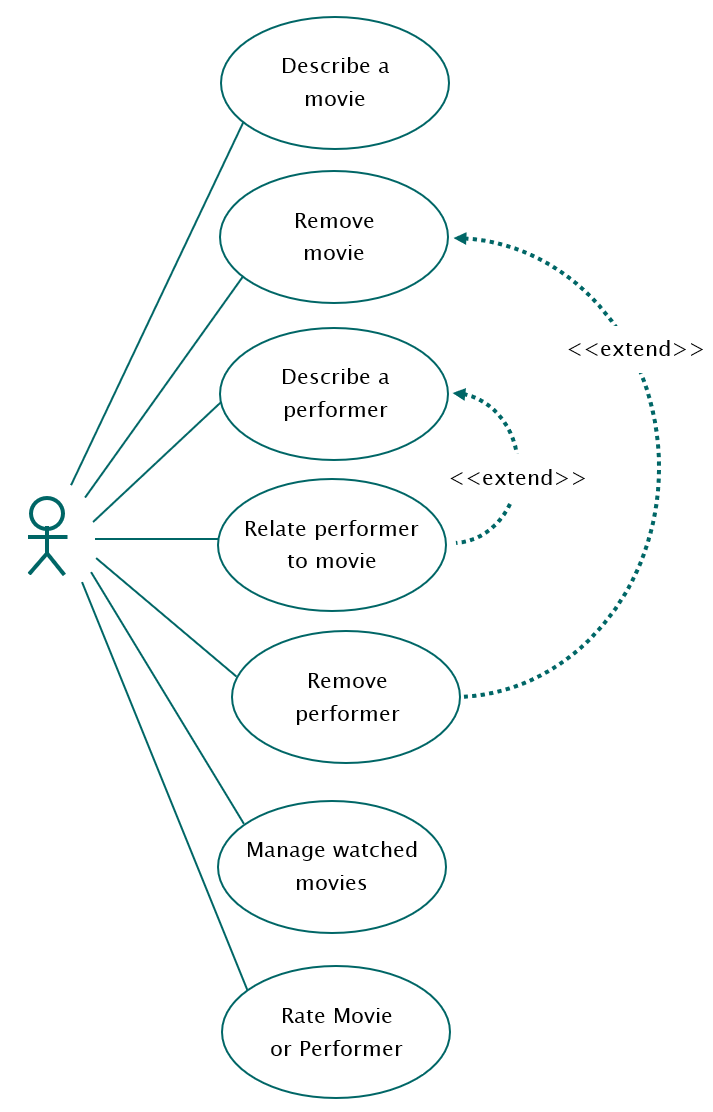
\includegraphics[width=.5\textwidth]{../images/ElAttarUseCase.png}
	\caption{Use Case Model for the Movie Manager application.}
	\label{fig:use-case-mm}
\end{figure}



\begin{figure}[H]
	\centering
	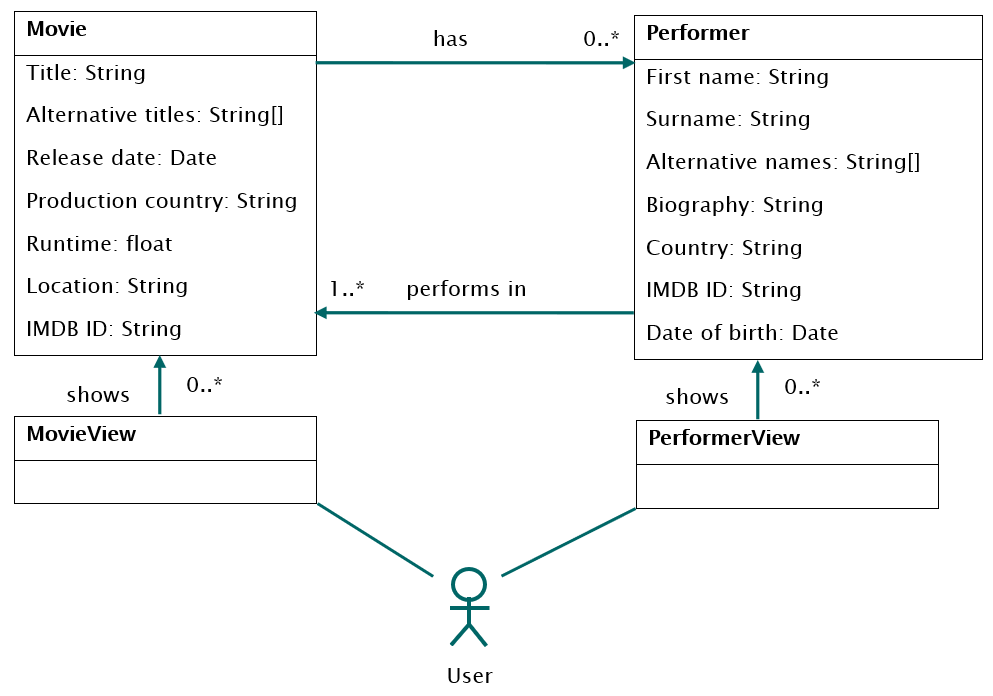
\includegraphics[width=.8\textwidth]{../images/ElAttarDomain.png}
	\caption{Domain Model for the Movie Manager application.}
	\label{fig:domain-mm}
\end{figure}



The HLATs for the Use Case \textit{Describe a Performer} are displayed in Table \ref{fig:hlats-mm}.
Each HLAT describes the necessary preconditions, inputs and the expected results of one User Scenario.
This information is extracted from Use Case description.

\begin{table}[H]
	\caption{HLATs for the Use Case \textit{Describe a performer} of the Movie Manager application.}	
	\centering
	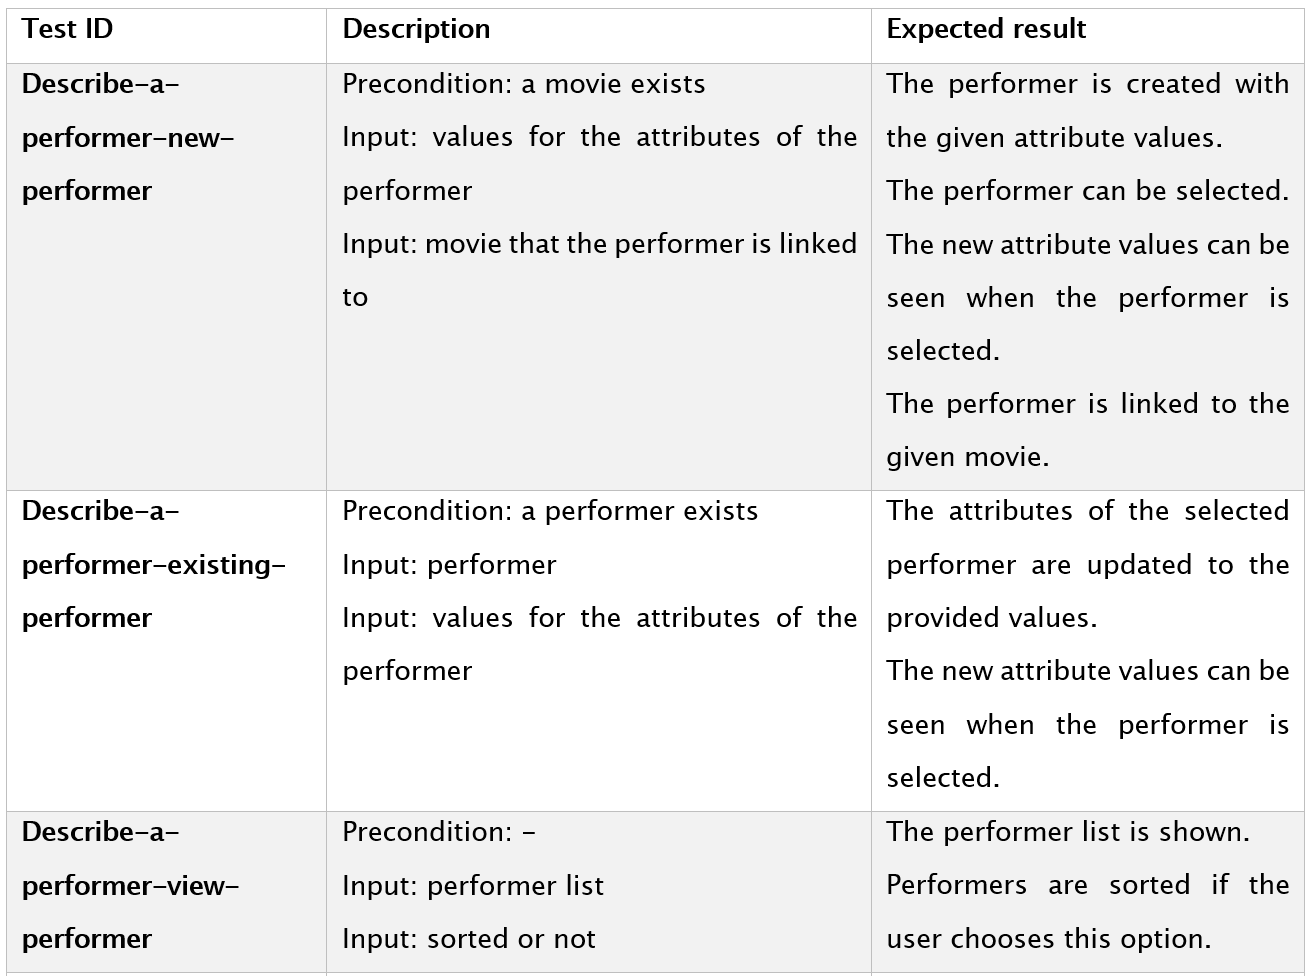
\includegraphics[width=.9\textwidth]{../images/ElAttarHLATs.png}
	\label{fig:hlats-mm}
\end{table}

In the next step a robustness diagram is created using the information from the Use Case Model and the Domain Model.
The robustness diagram for the Use Case \textit{Describe a movie} is shown in figure \ref{fig:robustness-mm} on the next page.
A robustness diagram contains the involved objects that communicate with the user.
These are called boundary objects.
An example for a boundary object is \textit{PerformerView} in figure \ref{fig:robustness-mm}.
It also contains control-objects like \textit{RelateToMovie} in figure \ref{fig:robustness-mm} that makes sure that a performer is related to at least one movie.
The last types of objects are the \textit{User} and the entities like \textit{Performer} or \textit{Movie} in figure \ref{fig:robustness-mm}.
The resulting robustness diagram is used to find new information for the domain diagram.
For example, CheckMovieRelations needs to find out whether the performer is linked to at least one existing movie.
Therefore, the domain model needs to include a list of related movies for each performer or the number of related movies.
In this example the first variant (a list of related movies) is used in the domain model.
So this specific information does not have to be added.
Overall the robustness analysis does not bring up any new information but possibly could for other examples which is why El-Attar and Smith have included it in their approach.


\begin{figure}[h!]
	\centering
	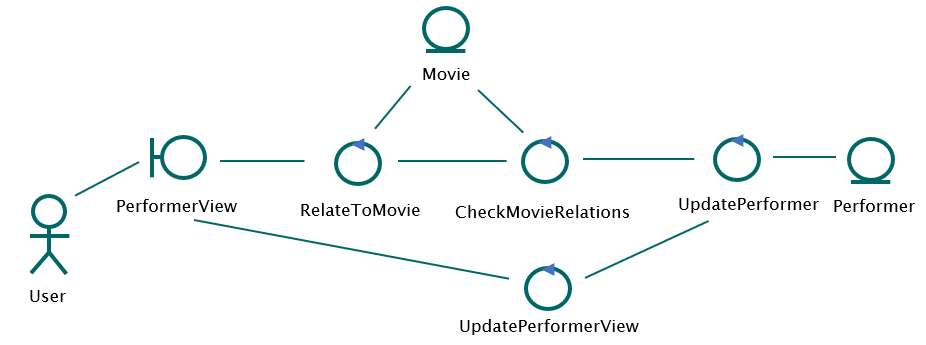
\includegraphics[width=.8\textwidth]{../images/ElAttarRobustness.png}
	\caption{Robustness Diagram for the Use Case \textit{Describe a performer} of the Movie Manager application.}
	\label{fig:robustness-mm}
\end{figure}



As last step executable acceptance tests are created for each HLAT.
These are created in the form of \textit{Fit-tables}.
For this example so called \textit{ActionFixtures} are chosen but \textit{RowFixtures} and \textit{ColumnFixtures} are also possible for this approach.
\textit{ActionFixtures} contain a Test ID in the first row.
Each of the following rows contains one action like entering a value or pressing a button.
The ActionFixtures for the three HLATs from table \ref{fig:hlats-mm} are displayed in the tables \ref{fig:eats1-mm}, \ref{fig:eats2-mm} and \ref{fig:eats3-mm} on the next page.
These Fit-tables are the final result of the approach.

\begin{table}[H]
	\caption{Executable Acceptance Tests for the scenario \textit{Describe a performer, new performer} of the Movie Manager application in form of an \textit{ActionFixture}. 
	A placeholder in the form of \textit{...} is used for entering the other possible attributes of a performer to reduce the size of the table.}
	\centering
	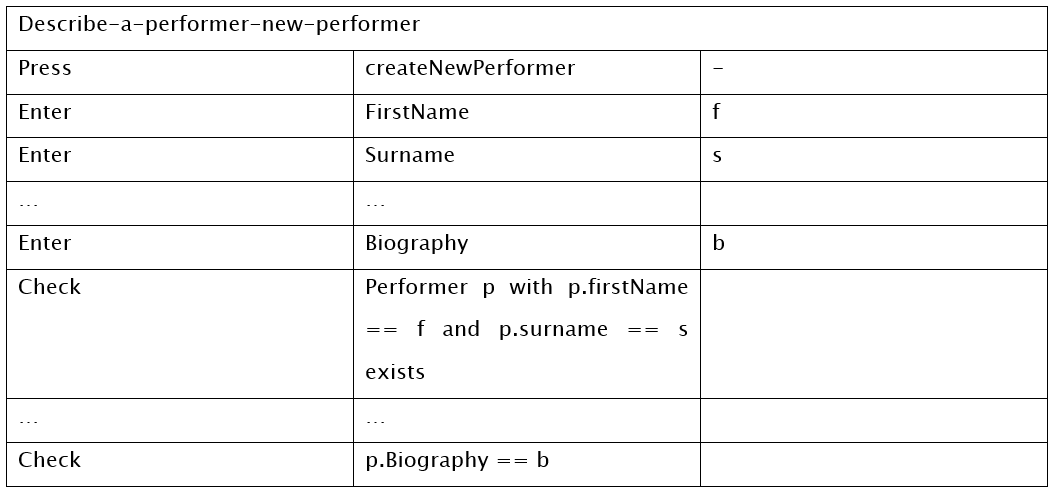
\includegraphics[width=.9\textwidth]{../images/ElAttarEATs1.png}
	\label{fig:eats1-mm}
\end{table}

\begin{table}[H]
	\caption{Executable Acceptance Tests for the scenario \textit{Describe a performer, existing performer} of the Movie Manager application in form of an \textit{ActionFixture}.
	A placeholder in the form of \textit{...} is used for entering the other possible attributes of a performer to reduce the size of the table.}
	\centering
	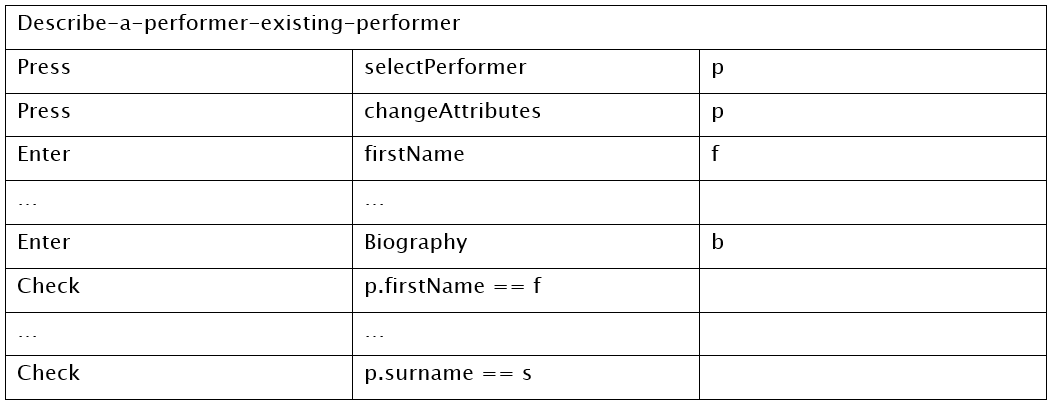
\includegraphics[width=.9\textwidth]{../images/ElAttarEATs2.png}	
	\label{fig:eats2-mm}
\end{table}

\begin{table}[H]
	\caption{Executable Acceptance Tests for the scenario \textit{Describe a performer, view performers} of the Movie Manager application in form of an \textit{ActionFixture}.
	A placeholder in the form of \textit{...} is used for entering the other possible attributes of a performer to reduce the size of the table.}
	\centering
	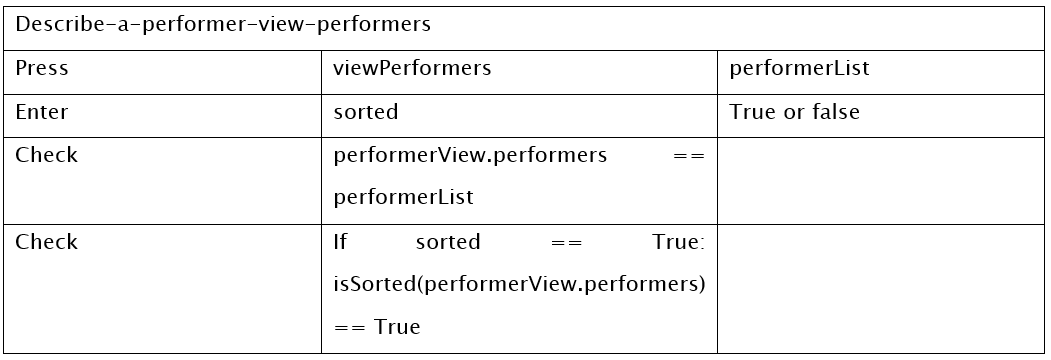
\includegraphics[width=.9\textwidth]{../images/ElAttarEATs3.png}
	\label{fig:eats3-mm}
\end{table}


\section{Approach 2: A web framework for test automation, user scenarios through user interaction diagrams}
\label{sec:longo}

\subsection{Description}

Longo et al. \cite{longo} create User Scenarios through User Interaction Diagrams (US-UIDs) which then are fully automatically converted into \textit{Fit-tables} that represent the test data for acceptance tests.
To run these acceptance tests a Fixture-Class is needed that connects the test data from the \textit{Fit-table} with the System-under-test.
The US-UIDs are created in a tool provided by the authors.
They contain functional data such as the involved objects, attributes and functions and also explicit User Scenarios provided by the customer.
The User Scenarios provide the test data and combined with the functional data, \textit{Fit-tables} can be automatically created.
The functional data represents the top row of the \textit{Fit-table} and the User Scenarios the specific values.
Figure \ref{fig:overview-longo} provides an overview over the steps of the approach.
The only step that is executed automatically is marked in this overview.
Each of the steps is explained in more detail in the following.

\begin{figure}[H]
	\centering
	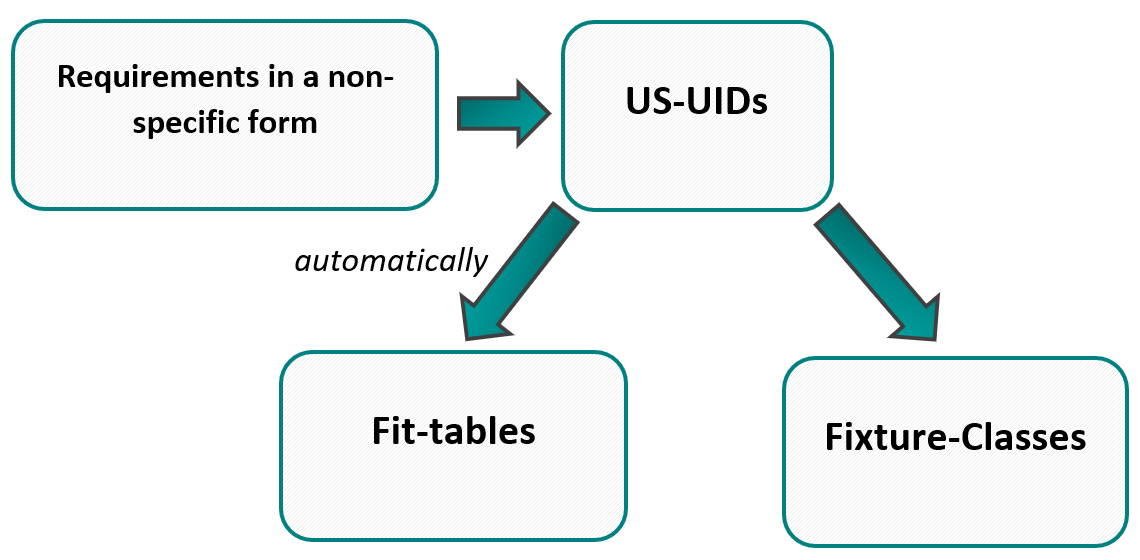
\includegraphics[width=.62\textwidth]{../images/LongoProcess.png}
	\caption{Overview of the steps in the approach of Longo et al.}
	\label{fig:overview-longo}
\end{figure}
\newpage
In the first step the US-UIDs are created.
This step is described in another work by the authors \cite{longo2}.
Each US-UID contains an explicit User Scenario provided by the customer.
The information about the User Scenario is extended by the developer by adding functional information.
For example, the User Scenario could provide a specific value for a variable.
Then the functional information for this value would be the name of the variable.
With this conjunction of explicit and functional values \textit{Fit-tables} can be automatically created.
The first row contains the functional information.
Each row after the first row represents a User Scenario and contains the given values for the functional information (objects, variables, etc.) given in the first row.

Each row can be used as one specific test case.
To execute these test cases a Fixture-Class is needed.
This class has to be written by the developers.
It creates an instance of the System-under-test and uses \textit{Setter methods} to provide the input from the \textit{Fit-table} to the System-under-test.
Through \textit{Getter methods} the resulting values of the System-under-test can be extracted to validate the success of the test.
For the evaluation step the results from the Getter methods are compared to the expected values from the \textit{Fit-table}.
If they are the same, the test was successful.

To evaluate their approach Longo et al. used their tool to automatically create executable acceptance tests from existing US-UIDs.
The developers of the software related to these US-UIDs already manually created test cases for the software.
In the evaluation the authors compared these manually created tests to the tests created by their tool.
To compare both of them the authors used the techniques \textit{code mutation} and \textit{lack of code}.
The technique \textit{code mutation} involved manipulating the values of an array in the software and \textit{lack of code} was executed by removing a class from the software.
By using both techniques failed tests could be found in both test sets.
The second technique also resulted for both test sets in tests that were not executable.
From these results the authors concluded that tests created with their approach can detect test cases that are \textit{successful}, \textit{failed} or \textit{not executable}.

\subsection{Application}

To illustrate the approach of Longo et al. the use case \textit{Describe a performer (new performer)} is used.
In the first step an US-UID has to be created that displays the explicit information of a User Scenario as well as the underlying functional information.
In this type of model the round boxes are states of the system.
The rectangles contain the User's Input whilst the free text in the round boxes describes the system's output.
Arrows are used to assign functional names to the data and to denote transitions between states.
The US-UID for the example is displayed in figure \ref{fig:us-uid-mm}.
In the beginning the performerList contains only the performers a, b and c with attributes e, f and g.
After the execution of the US-UID it also contains performer d with attributes x.


\begin{figure}[tbh]
	\centering
	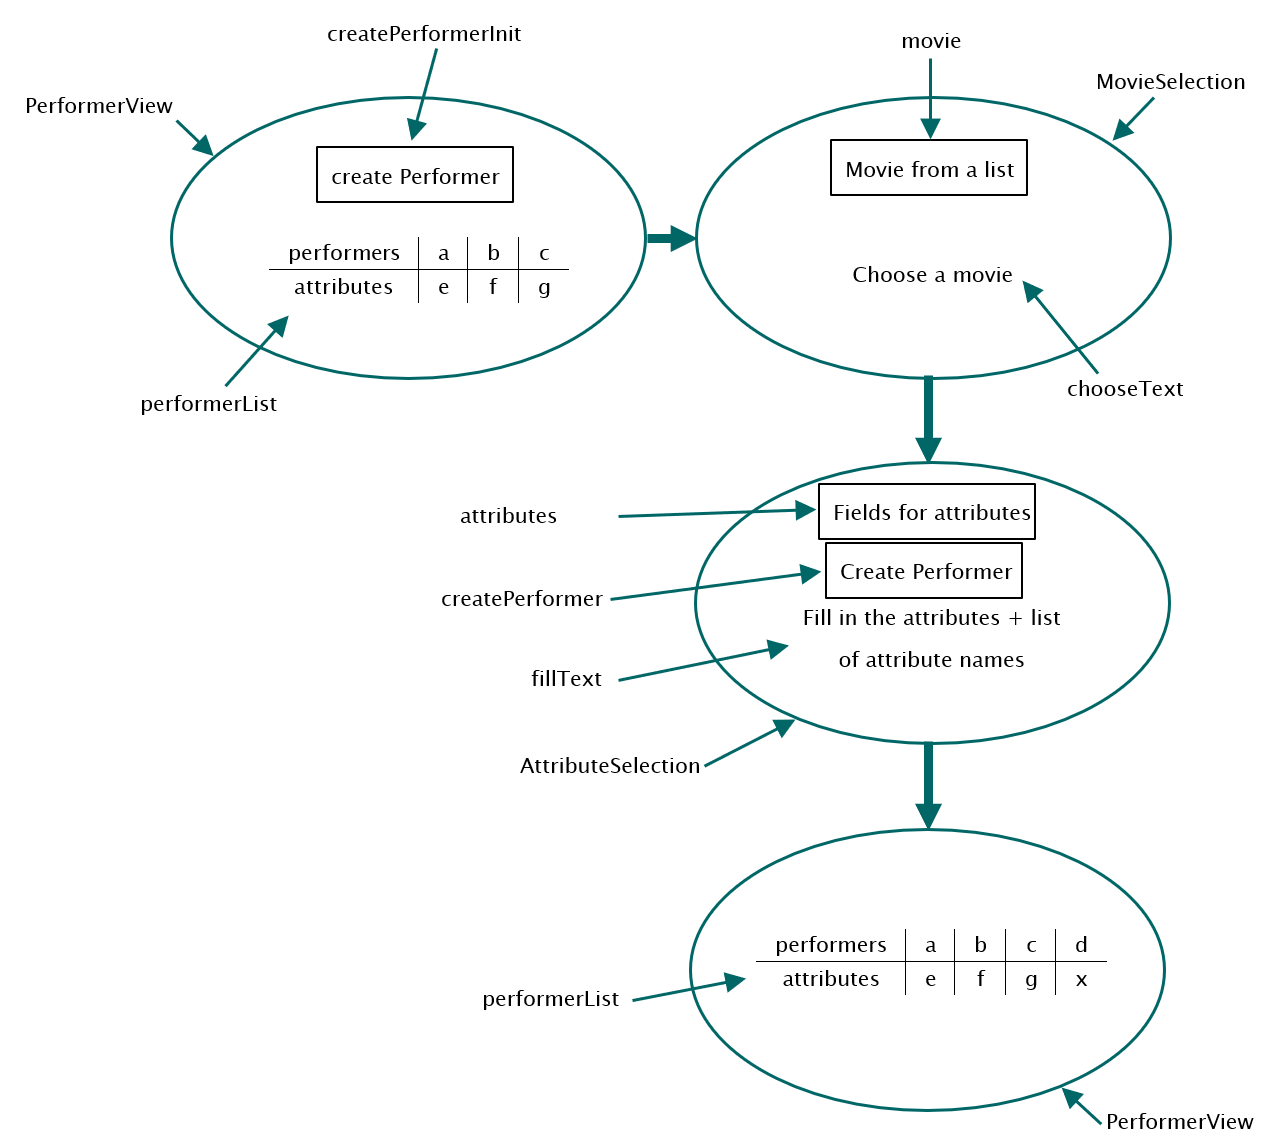
\includegraphics[width=.85\textwidth]{../images/US-UID.png}
	\caption{US-UID for the Use Case \textit{Describe a performer (new performer)} of the Movie Manager application.}
	\label{fig:us-uid-mm}
\end{figure}

In the next step the functional information from the US-UID needs to be connected to the real
objects and attributes of the \textit{System-under-test}. This is done in a Fixture-Class that is marked
with \textit{@Fixture}.
This class has to be written manually.
The data flow during the execution of acceptance tests with FitNesse and the role of the Fixture-Class in this process is described in section \ref{sec:topic_2_intro}.
Inputs are part of the functional data on the start of the arrows in the US-UIDs. 
For the first display of the US-UID PerformerView the Fixture-Class needs methods to move to the next display, to set the starting performer list and to choose
\textit{create Performer}.
Results have to be extracted from the System-under-test using Getter-Methods.
One such result is the updated performer list in the last state of the PerformerView.
This result can be compared to the expected result given in the US-UID.

In the final step a \textit{Fit-Table} is created.
This step is fully automatic with the tool of Longo et al. because it is only remodeling information from the US-UID.
The functional information is placed in the top row whilst the explicit data of the User Scenarios is stored in the following rows.
Each row represents an User Scenario.
The resulting \textit{Fit-table} for the example is displayed in table \ref{fig:fit-longo} on the next page.

\begin{table}[h!]
	\caption{\textit{Fit-table} for a specific User Scenario of the Use Case \textit{Describe a performer (new performer)} of the Movie Manager application. The expected results end with a question mark.}
	\centering
	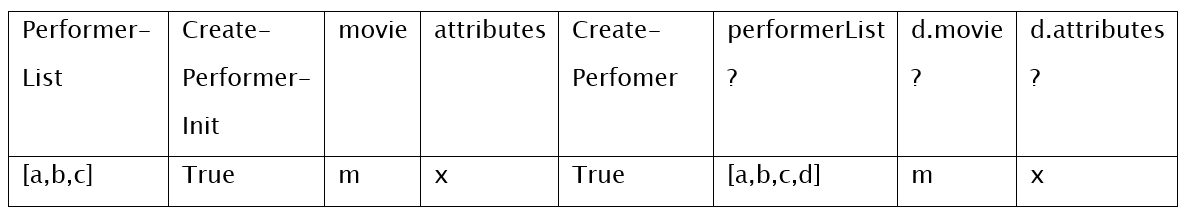
\includegraphics[width=\textwidth]{../images/LongoFit.png}

	
	\label{fig:fit-longo}
\end{table}

\newpage
\section{Comparison}
\label{sec:comparison}

As in the other chapters the approaches are compared in a synthesis matrix.

\renewcommand{\arraystretch}{1.5}
%	\begin{tabularx}{\textwidth}{>{\hsize=.2\hsize}X X}
%  		\textbf{1a} & Which artefacts and relations between artefacts are used in this approach? Which
%artefacts are created in the course of the approach? How are the artefacts characterized?
% \\
%  		\hline
%  		\textbf{1b} & What is required and/or input for the application of the approach? \\
%  		\hline
%  		\textbf{1c} & What steps does the approach consist of? Which information is used in which step
%and how? What are the results of the individual steps?
% \\
%  		\hline
%  		\textbf{2a} & Which usage scenarios are supported by the approach? \\
%  		\hline
%  		\textbf{2b} & Which stakeholders are supported by the usage scenarios? \\
%  		\hline
%  		\textbf{2c} &  Which knowledge areas from SWEBOK can be assigned to the usage scenarios? \\
%  		\hline
%  		\textbf{3a} & What tool support is provided for the approach? \\
%  		\hline
%  		\textbf{3b} & Which steps of the approach are automated by a tool? Which steps are supported
%by a tool, but still have to be executed manually? Which steps are not supported
%by a tool?
% \\
%  		\hline
%  		\textbf{4a} & How was the approach evaluated? \\
%  		\hline
%  		\textbf{4b} & What are the (main) results of the evaluation? \\
%  		\end{tabularx}
 
\begin{small} 		
\begin{longtable}[h]{p{0.45cm}|p{0.425\textwidth}|p{0.425\textwidth}}
	\caption{Synthesis matrix}
	\label{tab:blub}
	\\    %%%%<===
	\hline
  	\textbf{No.} & \textbf{Approach 1} & \textbf{Approach 2}\\
  	\hline
  		 1a) & Initial artefacts: \textbf{Use Case and Domain Models} are used to create high level acceptance tests and robustness diagrams 
\textbf{Robustness diagrams} combine the information from the use cases and the domain model. During the creation of the robustness diagrams for the use cases objects and attributes may be identified that are missing in the domain model. The domain model is updated with this missing information.
\textbf{High level acceptance tests (HLATs)} deliver an informal description of acceptance tests. They are tables and use keywords that are chosen by their creator. For each flow of a use case from the Use Case model a HLAT is created.
\textbf{Fit-tables} are a form of executable acceptance tests that can be automatically executed by the tool FitNesse. For each HLAT a Fit-table is created using the information about the control flow in the respective robustness diagram.
 & \textbf{User Scenarios through User Interaction Diagrams (US-UIDs)} show the interaction during a User Scenario. They include User-Input, System-Output, states of interaction and transitions between states.
\textbf{Fit-tables} are a form of executable acceptance tests that can be automatically executed by the tool FitNesse. The Fit-tables in this approach need a specific Fixture-Class for each Use Case that allows the flow of information between the Fit-table and the System-under-test.
 \\
 \hline
  1b) & \begin{itemize}
  		 \item Use Case Model \item Domain Model
\end{itemize}  		  & Requirements in a non-specific type \\
	\hline
  1c) & As initial artefacts Use Case models and Domain models are used.
In the first step a HLAT is created for each flow of each use case from the Use Case model. The information about the preconditions, inputs and triggers for the HLATs gets extracted from the domain model.
The second step is the creation of robustness diagrams for the use cases from the Use Case model. These diagrams also include the objects from the domain model and model the communication between those in the specific use case. If objects or attributes are found in this step that are necessary but not yet part of the domain model, they are added to the domain model. All the other models are updated to fit the domain model. In the last step a Fit-table is created for each HLAT using the control flow that can be seen in the robustness diagram. 
Finally the created Fit-tables can be combined with the Use Case from the Use Case model that they belong to.
 & In the first step the US-UIDs are created by using the known requirements.
The customer delivers the User Scenario and the developer add the functional information for the data used in the scenario.
The Fit-tables are created automatically from the information of the US-UIDs. This step is done by the web framework.\\
\hline
  2a) & Business Analysts receive a systematic approach to create acceptance tests in the Fit-syntax.
Customers receive a product that fits their requirements.
Developers receive acceptance tests that they can use to determine which requirements of the customers they have already implemented and which they have to work on.
 & Customers and developers receive an approach to develop acceptance tests together that include User scenarios provided by the customer.
Developers receive acceptance tests that they can use to determine which requirements of the customers they have already implemented and which they have to work on.
 \\
  \hline
  		 2b) & 
  		 	\begin{itemize}
  		 		\item Developer 
  		 		\item Customer 
  		 		\item  Business Analyst
			\end{itemize}  		 
			& \begin{itemize}
  		 		\item Developer 
  		 		\item Customer
				\end{itemize}\\
	 \hline
  		 2c) & Developer: Software Construction (Test-driven development) \newline
Business Analyst \& Customer: Software Testing
 & Customer/Developer: Software Requirements, Software Testing \newline
Developer: Software Construction (Test-Driven Development)
 \\
  		\hline
  		 3a) & The authors provide the tool UCAT in which Use Case Models and Fit-tables can be created and linked. The created Fit-tables can be automatically executed using FitNesse. & A web framework is provided by the authors in which US-UIDs can be created and converted to Fit-tables. These Fit-tables can be executed with FitNesse. \\
  	 \hline
  		 3b) & The tool UCAT serves as an editor to create Use Case models and Fit-tables. Those two artefacts can also be linked in UCAT.
Every other step in the creation of the acceptance tests is done without tool support.
No step of the approach is done automatically.
 & The creation of the US-UIDs is supported by the web framework which serves as an editor.
Converting the US-UIDs to Fit-tables is done fully automatically by the web framework.
Every other step in the creation of the acceptance tests is done without tool support.
 \\
  \hline
  4a) & 
  	\begin{itemize} 
  		\item Case study with an application (RestoMapper)
		\item	No real evaluation 
	\end{itemize}
 & The authors created tests automatically from existing US-UIDs of an existing application using their approach.
The resulting test set was compared to an existing test set that was created manually.
The code of the application was manipulated using code mutation and lack of code.
For the method code mutation the values of an array were changed manually. For lack of code a class was deleted.
 \\
  \hline
  		 4b & The approach can be applied on an example.
Otherwise no evaluation results because the authors state that an evaluation is beyond the limitations of their work.
The reason for this is that the quality of the created tests in this approach highly depends on the experience and skill of the person executing the approach.
 & Code mutation and lack of code resulted for both test sets in failed tests.
Lack of code also resulted in not executable tests.
The authors concluded that the tests created by their approach can successfully classify tests as successful, failed or not executable.
 \\
  \hline
\end{longtable}
\end{small}

Both approaches provide a possible way to create acceptance tests that are executable with the tool \textit{FitNesse}.
El-Attar and Smith utilize use case models and domain models as their initial data while Longo et al. only need a non-specific description of the use cases.
Generally El-Attar and Smith use more artefacts as their approach needs use case models, domain models, high-level acceptance tests and robustness diagrams as intermediate steps to the final representation of the executable acceptance tests.
In the approach of Longo et al. only US-UIDs need to be created which are then automatically converted to \textit{Fit-tables}.
In contrary to El-Attar and Smith the approach of Longo et al. requires the creation of some code in the process:
This is the case because the used \textit{Fit-tables} differ between the two approaches.
While El-Attar and Smith use the specific table types ActionFixture, RowFixture and ColumnFixture, Longo et al. use easier \textit{Fit-tables} that are connected to the System-under-test via a Fixture-Class.
This Fixture-Class has to be written manually.

Both approaches provide a tool to combine artefacts with the resulting acceptance tests which helps traceability.
For both approaches the creation of the executable acceptance tests is still mostly or completely manual.
While the approach of El-Attar and Smith uses no automation during the creation of the executable acceptance tests, the last step of the approach of Longo et al. is fully automatically.
This is possible because the US-UIDs created in the approach of Longo et al. are a different way to display the information of a \textit{Fit-table} and therefore can be directly converted to a \textit{Fit-table}.
The execution of the final acceptance tests is fully automatic for both approaches.

Both approaches involve customer and developers as stakeholders.
The customer delivers the User Scenarios and receives (because of the development of acceptance tests) potentially a final product that is closer to his needs.
The developers receive automatically executable tests that help them during the development process to determine which requirements are already satisfied and which still need to be implemented.
While in the approach of Longo et al. the creation process of the acceptance tests is done by the customer and the developers together, in the approach of El-Attar and Smith a Business Analyst is responsible for this process.

El-Attar and Smith only visualize their approach through an example and state that the approach cannot be validated in their work because it is beyond the limitations of their work.
The reason for this is that all the steps to create the acceptance tests are done manually and therefore depend on the experience and skill of the analyst performing the steps.
Longo et al. include a small evaluation in their work.
They compare the tests created by their approach to tests that are created without guidelines from the same US-UIDs.
During the testing phase they conclude that the tests created by their approach can be classified as \textit{successful}, \textit{failed} or \textit{not executable}.
Also changes in the source code of the System-under-test resulted in failed tests for both of the test sets which leads the authors to the conclusion that both the tests created without guidelines as well as the tests created with their approach can detect fails in the System-under-test.


\section{Conclusion}
\label{sec:topic_2_conclusion}

The literature search showed that creating acceptance tests that are automatically executable with the specific tool \textit{FitNesse} is not a widely researched topic in the literature.
However, approaches exist that differ in their process to create tests.
Two of these approaches were presented in this chapter:

The approach by El-Attar \& Smith is aimed at larger projects and therefore, might not be useful for smaller products.
It requires the creation of a lot of UML models.
If an analyst exists that has experience in creating these models and at least a few of the used models are created anyway in the engineering process, then this approach might be useful.

The second approach by Longo et al. could be used for smaller projects where the customer is heavily involved.
The customers have to be involved because they have to provide the User Scenarios in this approach.
The approach is heavily dependent on the creation of US-UIDs that contain the information of Fit-tables in a different (possibly better) way.
If the developers and customers prefer US-UIDs over Fit-tables and they want to use User Scenarios, this approach might be useful.

Overall, in the considered approaches the creation of acceptance tests is a process that is highly dependent on the experience and skill of the persons involved.
Once the executable tests are created they are an easy way to measure how well the requirements of the customer are implemented.

